%%%%%%%%%%%%%%%%%%%% author.tex %%%%%%%%%%%%%%%%%%%%%%%%%%%%%%%%%%%
%
% sample root file for your "contribution" to a contributed volume
%
% Use this file as a template for your own input.
%
%%%%%%%%%%%%%%%% Springer %%%%%%%%%%%%%%%%%%%%%%%%%%%%%%%%%%%%%%%%%


% RECOMMENDED %%%%%%%%%%%%%%%%%%%%%%%%%%%%%%%%%%%%%%%%%%%%%%%%%%%
\documentclass[graybox]{svmult}

% choose options for [] as required from the list
% in the Reference Guide

\usepackage{mathptmx}       % selects Times Roman as basic font
\usepackage{helvet}         % selects Helvetica as sans-serif font
\usepackage{courier}        % selects Courier as typewriter font
\usepackage{type1cm}        % activate if the above 3 fonts are
                           % not available on your system

\usepackage{makeidx}         % allows index generation
\usepackage{graphicx}        % standard LaTeX graphics tool
                             % when including figure files
\usepackage{multicol}        % used for the two-column index
\usepackage[bottom]{footmisc}% places footnotes at page bottom

%custom package
\usepackage{mathtools}

% see the list of further useful packages
% in the Reference Guide

\makeindex             % used for the subject index
                       % please use the style svind.ist with
                       % your makeindex program

%%%%%%%%%%%%%%%%%%%%%%%%%%%%%%%%%%%%%%%%%%%%%%%%%%%%%%%%%%%%%%%%%%%%%%%%%%%%%%%%%%%%%%%%%

\begin{document}

\title{Global search algorithms for one-dimensional multiextremal optimization problems with nonlinear constraints}
% Use \titlerunning{Short Title} for an abbreviated version of
% your contribution title if the original one is too long
\author{Name of First Author and Name of Second Author}
% Use \authorrunning{Short Title} for an abbreviated version of
% your contribution title if the original one is too long
\institute{Name of First Author \at Name, Address of Institute, \email{name@email.address}
\and Name of Second Author \at Name, Address of Institute \email{name@email.address}}
%
% Use the package "url.sty" to avoid
% problems with special characters
% used in your e-mail or web address
%
\maketitle

\abstract{The chapter considers a method for reduction of a constrained problem to an
unconstrained one, so called \emph{index method}. This method, unlike the classical penalty function
one, allows avoiding the problem of the parameter selection (like the penalty coefficients for the
constraints) and also allows solving the problems with so called partially defined constraints,
which could not be solved by any other method. The serial and parallel algorithms for solving
univariate problems are considered.}

\keywords{multiextremal optimization, nonconvex constraints, index method, parallel
algorithms}

\section{Problem statement}
In the present chapter, the one-dimensional problems of the constrained optimization will
be considered. Let $\varphi(x)$ and $g_j(x)\le 0,1\le j\le m$ be the real functions defined in a closed interval $[a,b]$ of the real axis. It is requires to find the values $x^*$ satisfying the condition
\begin{equation}
  \label{eq4:problem}
  \varphi(x^*)=\min\{\varphi(x):x\in [a,b], g_j(x)\le 0,1\le j\le m\}
\end{equation}

As before, the objective function $\varphi$ (hereinafter denoted also as $g_{m+1}$) and the left parts of the constraints $g_j(x)\le 0,1\le j\le m$ re assumed to satisfy \emph{Lipschitz condition} with the corresponding constants $L_j,1\le j\le m+1$, namely:
\begin{equation}
  |g_j(x_1)-g_j(x_2)|\le L_j|x_1-x_2|,1\le j\le m+1,x_1,x_2\in [a,b]
\end{equation}

\example{
\label{ex4:problem}
Let us consider a problem of type \eqref{eq4:problem} where $x\in [0.6;2.2],m=2$,
\begin{gather*}
  \varphi(x)=\cos(18x-3)\sin(10x-7)+1.5, \\
  g_1(x)=\exp(-x/2)\sin(6x-1.5), \\
  g_2(x)=|x|\sin(2\pi x-0.5).
\end{gather*}
he exact solution of the problem is $x^*=2.0795,\varphi(x^*)=0.565$. The graphs of the functions $g_1(x),g_2(x)$,and $\varphi(x)$ are presented in Fig. \ref{fig:4_1}.
\begin{figure}[h]
  \label{fig:4_1}
  \centering
  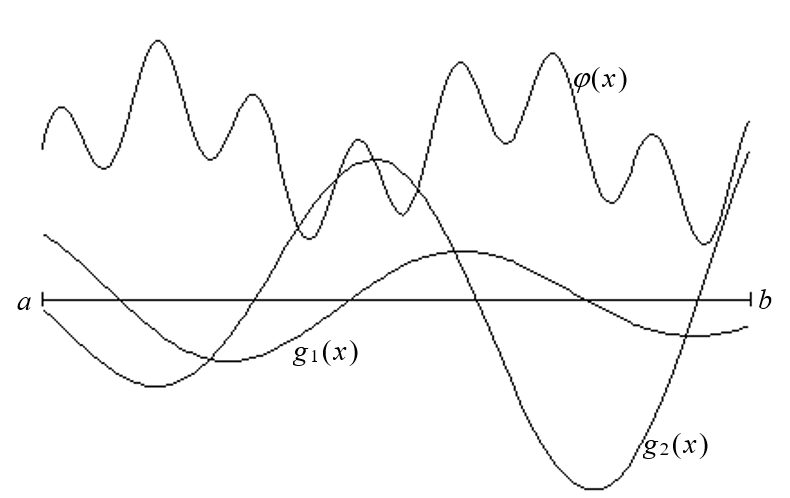
\includegraphics[width=0.8\textwidth]{figures/4_1.png}
  \caption{One-dimensional global optimization problem}
\end{figure}
}

\section{Partial computability and index scheme of the account of constraints}
Problem \eqref{eq4:problem} can be considered in the statement when each function $g_j,1\le j\le m+1$ is defined and computable only in the corresponding subdomains $Q_j\subset [a,b]$ where
\begin{equation}
  \label{eq4:q}
  Q_1=[a,b],Q_(j+1)=\{x\in Q_j:g_j(x)\le 0\},1\le j\le m.
\end{equation}

For example, in the optimal design problems some characteristics of the technical systems may appear to be undefined if the conditions of the system functioning represented by a part of the constraints of problem \eqref{eq4:problem} are not fulfilled.

Taking into account conditions \eqref{eq4:q}, initial problem \eqref{eq4:problem} can be represented in the form
\begin{equation}
  \label{eq4:problem2}
  \varphi(x^*)=\min\{g_{m+1}(x):x\in Q_{m+1}\}.
\end{equation}

For the purposes of further treatment, let us introduce a classification of the points $x$ in the search domain $[a,b]$ using an index $\nu=\nu(x)$ where $\nu-1$ is the number of constraints, which are fulfilled in this point. Formally, the index $\nu$ is defined by the conditions
\begin{equation}
  \label{eq4:condition}
  g_j(x)\le 0,1\le j \le \nu-1,g_\nu(x)>0,
\end{equation}
(the last inequality is inessential  if $\nu=m+1$) and it satisfies the inequalities
\begin{displaymath}
  1\le\nu=\nu(x)\le m+1.
\end{displaymath}
The problem of example \ref{ex4:problem} assuming a partial computability of the functions is presented in Fig. \ref{fig:4_2}. The arcs of the restrictions $g_1(x),\:g_2(x)$, and of the objective function $\varphi(x)$ defined in the corresponding subdomains $Q_j$ from \eqref{eq4:q} are shown. The point $x^1$ with the index $\nu(x^1)=1$, the point $x^2$ with the index $\nu(x^2)=2$, and the point $x^3$ with the index $\nu(x^3)=3$ are shown also.

\begin{figure}[h]
  \label{fig:4_2}
  \centering
  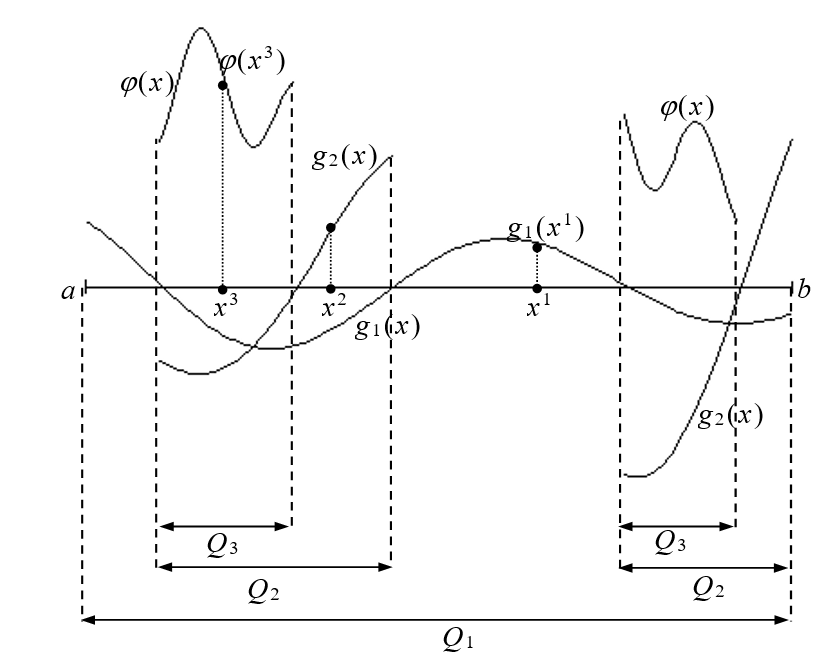
\includegraphics[width=0.8\textwidth]{figures/4_2.png}
  \caption{A problem with partially computable functions}
\end{figure}

This classification generates the function
\begin{equation}
  \label{eq4:fx}
  f(x)=g_\nu(x),\nu=\nu(x),
\end{equation}
defined and computable everywhere in $[a,b]$. Its value at a point $x$ is either the value of the left part of the constraint violated at this point (the case $\nu\le m$)  or the value of the objective function (the case $\nu=m+1$). Therefore, the determination of the value of $f(x),\:x\in[a,b]$  is reduced to a successive computations of the values of $g_j(x), 1\le j\le \nu=\nu(x)$, i.e., the next value $g_{j+1}(x)$ is calculated in the case when $g_j(x)\le 0$ only. The computational process finishes either as a result of the fulfillment of the inequality $g_j(x)>0$ or as a result of achievement of the value $\nu(x)=m+1$.

The described procedure called a \emph{trial} at the point $x$ forms the index $\nu$ of this point automatically. The pair of values
\begin{equation}
  \label{eq4:trial}
  z=f(x)=g_\nu(x),\nu=\nu(x)
\end{equation}
generated by the trial at the point $x\in[a,b]$ is called the \emph{trial result}.

The graph of the function $f(x)$ from \eqref{eq4:fx}, which consists of the arcs of the constraints $g_1(x),\:g_2(x)$, and of the objective function $\varphi(x)$ taken from Example \ref{ex4:problem} is shown in Fig. \ref{fig:4_3}.

\begin{figure}[h]
  \label{fig:4_3}
  \centering
  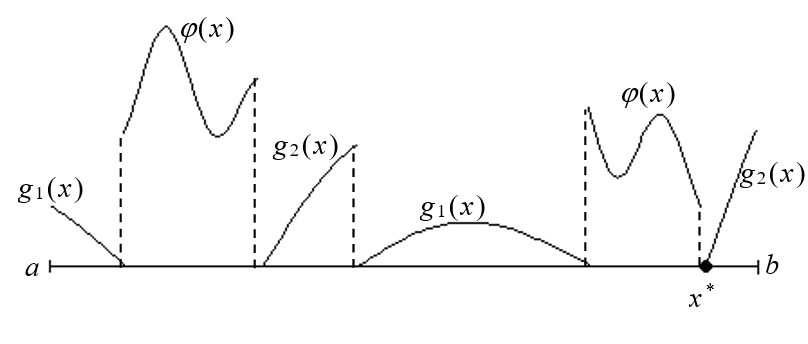
\includegraphics[width=0.8\textwidth]{figures/4_3.png}
  \caption{An ''index'' function}
\end{figure}

Since in the general case the problem \eqref{eq4:problem2} may have no solution (i.e., the feasible subdomain $Q_{m+1}$ might appear to be empty because of the incompatibility of the constrains) an auxiliary problem always having a solution is associated with it. Since conditions \eqref{eq4:condition} are equivalent to the conditions
\begin{displaymath}
  x\in Q_\nu,x\not\in Q_{\nu+1},
\end{displaymath}
this auxiliary problem can be written in the form
\begin{equation}
  \label{eq4:problem3}
  g_M^*=g_M(x_M^*)=\min\{g_M(x):x\in Q_M\},
\end{equation}
where $M$ is the greatest possible value of the index i. e.
\begin{equation}
  1\le M=\max\{\nu(x):x\in[a,b]\}\le m+1
\end{equation}
Since the set $Q_M$ is always nonempty, problem \eqref{eq4:problem3} always has a solution. When $M=m+1$ the solution $x^*=x^*_m+1$  is also the solution of the initial problem \eqref{eq4:problem}. When $M<m+1$ the inequality $g_M^*<0$ fulfilled necessarily can be used as an indicator of the incompatibility of the constraints.

The main idea of the index approach is to reduce the constrained problem \eqref{eq4:problem3} to a unconstrained one
\begin{displaymath}
  \psi(x^*)=\min\{\psi(x):x\in[a,b]\},
\end{displaymath}
where
\begin{equation}
  \psi(x)=
  \begin{cases}
    g_\nu(x)/L_\nu, & \nu < M, \\
    (g_M-g_M^*), & \nu=M.
  \end{cases}
\end{equation}

As a result, the arcs of $\psi(x)$ will be Lipschitzian with the constant $L=1$ in each subdomain $Q_\nu,1\le\nu\le M$. A graph of the function $\psi(x)$ for the example (\ref{ex4:problem}) is presented in Fig. \ref{fig:4_4}. This new function will have discontinuities of the first type at the boundary points of the subdomains $Q_\nu$ from \eqref{eq4:q}. Nevertheless, one can estimate the global minimizer $x^*_M$ using the results of $k$ trials for \eqref{eq4:trial} at the points $x_1,\dots, x_k$ in $[a,b]$ (see \cite{3}).

Indeed, as follows from Lipschitz condition
\begin{equation}
  \label{eq4:lip_opt_est}
  x^*_M\in\{x\in[a,b]:|x-x^i|\ge\psi(x^i),1\le i\le k\}.
\end{equation}

For example, a case for $k=4$ is presented in Fig. \ref{fig:4_4}. The union of the segments highlighted with a bold line in Fig. \ref{fig:4_4} is a complement of the set from the right hand side of \eqref{eq4:lip_opt_est} and does not include the optimum point.
\begin{figure}[h]
  \label{fig:4_4}
  \centering
  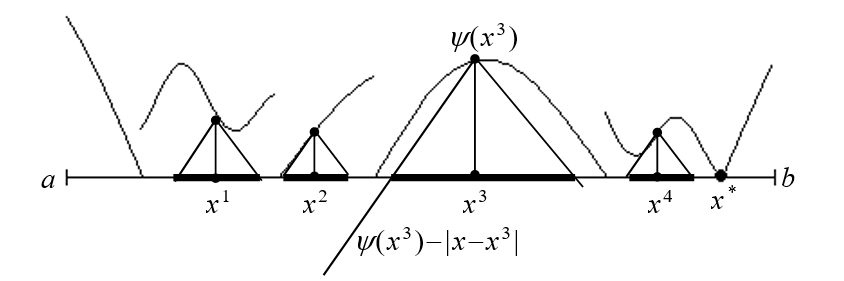
\includegraphics[width=0.8\textwidth]{figures/4_4.png}
  \caption{An estimate of the optimum point}
\end{figure}

Note that the greatest index $M$, the values of Lipschitz constants $L_\nu, 1\le \nu\le M$, and the value of $g_M^*$ are the unknowns. However, these problems can be overcome by means of using instead of them the adaptive estimates of these values obtained in the course of solving the problem on the base of trial results.

Having introduced all necessary concepts, let us turn to the description of the index algorithm.

\section{The index global search algorithm}
The first trial is executed at an arbitrary internal point $x_1\in(a,b)$. The selection of any subsequent trial point $x^{k+1},k\ge 1$ is determined by the following rules.

\emph{Rule 1.} Renumber the points $x^1,...,x^k$ of the preceding trials by the lower indices in ascending order of coordinate values, i.e.
\begin{equation}
  \label{eq4:search_data}
  0=x_0<x_1<\dots <x_k<x_{k+1}=1,
\end{equation}
and juxtapose to them the values $z_i=g_\nu(y(x_i)), \; \nu=\nu(x_i), \; 1
\leq i \leq k$, from \eqref{eq4:fx}; the points $x_0=0$ and
$x_{k+1}=1$ are introduced additionally for the convenience  of further notation (the values $z_0$ and $z_{k+1}$ are not defined).

\emph{Rule 2.} Classify the indices $i, \; 1 \leq i \leq k$, of the trial points from set \eqref{eq4:search_data} according to the number of the problem constraints fulfilled at these points, by constructing the sets
\begin{equation}
  I_\nu =\left\{i:1 \leq i \leq k, \; \nu=\nu(x_i) \right\}, \; 1 \leq \nu \leq m+1,
\end{equation}

containing the numbers of all the points $x_i, \; 1 \leq i \leq k$, with
the same values of $\nu$. The end points $x_0=0$ and $x_{k+1}=1$ are
interpreted as the ones having indices equal to zero. An additional set,
$I_0=\left\{0,k+1\right\}$, corresponds to them.

\emph{Rule 3.} Determine the maximum value of the index:
\begin{equation}
  M=\max\left\{\nu(x_i), \; 1 \leq i \leq k \right \}.
\end{equation}

\emph{Rule 4.} Compute the current lower estimates,
\begin{equation}
  \label{eq4:lip_est}
  \mu = \max\left\{ \frac{\left|z_i-z_j\right|}{ x_i - x_j }, \; i,j \in I_\nu, \; i>j \right\},
\end{equation}
for the unknown Lipschitz constants $L_\nu$ of the functions $g_\nu(y),1
\leq \nu \leq m+1$. If a set $I_\nu$ contains less than two elements, or
if $\mu_\nu$ is equal to zero, then assume $\mu_\nu=1$. As follows from \eqref{eq4:lip_est}, the estimates $\mu_\nu$ are non-decreasing starting from the moment when \eqref{eq4:lip_est} generates a positive value $\mu_\nu$.

\emph{Rule 5.} For all nonempty sets $I_\nu, \; 1 \leq \nu \leq m+1$, compute the estimates
\begin{equation}
  \label{eq4:mu_const}
  z_\nu^\ast = \left\{
  \begin{array}{lr}
    0, & \nu < M,\\
    \min\{ g_\nu(y(x_i): i\in I_\nu \}, & \nu = M.
  \end{array}
  \right.
\end{equation}

\emph{Rule 6.} For each interval ($x_{i-1},x_i), \; 1 \leq i \leq k+1,$ compute the \textit{characteristics} $R(i)$:
\begin{gather}
  \label{eq4:characteristic}
  R(i)=2\Delta_i-4\frac{z_i-z_\nu^\ast}{r_\nu \mu_\nu}, \; \nu=\nu(x_i)>\nu(x_{i-1}), \nonumber \\
  R(i)=\Delta_i+\frac{(z_i-z_{i-1})^2}{r_\nu^2 \mu_\nu^2\Delta_i}-2\frac{z_i+z_{i-1}-2z_\nu^\ast}{r_\nu \mu_\nu}, \;  \nu=\nu(x_i)=\nu(x_{i-1}),\\
  R(i)=2\Delta_i-4\frac{z_{i-1}-z_\nu^\ast}{r_\nu \mu_\nu}, \; \nu=\nu(x_{i-1})>\nu(x_i), \nonumber \\
  \Delta_i=x_i - x_{i-1} \nonumber
\end{gather}
The values $r_\nu>1, 1\le\nu\le m+1$ are the parameters of the algorithm. An appropriate choice of the values $r_\nu$ allows using the products $r_\nu\mu_\nu$ as the estimates of Lipschitz constants $L_\nu, 1\le\nu\le m+1$.

\emph{Rule 7.} Find the interval $(x_{t-1},x_t)$ with the maximum characteristic
\begin{equation}
\label{eq4:MaxR}
R(t)=\max{\left\{R(i): 1 \leq i \leq k+1\right\}}.
\end{equation}

\emph{Rule 8.} Make the next trial at the midpoint of the interval
$(x_{t-1},x_t)$ if the indices of the points $x_{t-1}$ and $x_t$  are not the same, i.e.
\[
x^{k+1} = \frac{x_t + x_{t-1}}{2}, \; \nu(x_{t-1}) \neq \nu(x_t).
\]
Otherwise, make the trial at the point
\begin{equation}
\label{eq4:next_point}
x^{k+1} = \frac{x_t+x_{t-1}}{2} - \frac{z_t-z_{t-1}}{2r_\nu\mu},\; \nu=\nu(x_{t-1})=\nu(x_t).
\end{equation}

The described rules can be supplemented with the termination condition, finalizing the iterations of the method if
\begin{equation}
\label{eq4:stop_cond}
  x_t - x_{t-1}\le\epsilon
\end{equation}
where t from \eqref{eq4:MaxR} and $\epsilon>0$ is the predefined accuracy of the optimization.

Let us formulate the conditions of convergence for the algorithm in the form of the following theorem.
\begin{theorem}
Let the considered index algorithm be applied to the solving of problem \eqref{eq4:problem} and the following conditions be satisfied:
\begin{enumerate}
  \item each function $gj, 1\le j\le m+1$ satisfies Lipschitz condition with the constant $L_j$ in the interval $[a,b]$, i.e.,
  \[
  |g_j(x_1)-g_j(x_2)|\le L_j|x_1-x_2|,1\le j\le m+1,x_1,x_2 \in[a,b]
  \]
  \item the following inequalities hold for the quantities $\mu_\nu$ from \eqref{eq4:lip_est} starting from some step
  \[
  r_\nu\mu_\nu > 2L_\nu,1\le\nu\\le m+1.
  \]
\end{enumerate}

Then the set of the limit points of the sequence $\{x_k\}$ generated by the index algorithm coincides with the set of solutions of problem \eqref{eq4:problem} with $\epsilon=0$ and termination criterion \eqref{eq4:stop_cond}. In addition, the index of each limit point equals to $M$ and the convergence to any limit point $\overline{x}$  is bilateral if $\overline{x}\not=a$ and $\overline{x}\not=b$.
\end{theorem}

This theorem is given without a proof, which can be found, for example, in \cite{}[1, 2]. Various modifications of this algorithm and the corresponding theory of convergence are given in \cite{}[5–10].

\textbf{The results of the experiment.} Let us consider a problem from Example (\ref{ex4:problem}) as an illustration. Under assumption of partial computability the arcs of the problem functions corresponding to the domains $Q_j, 1\le j\le 3$, from \eqref{eq4:q} are presented in Fig. \ref{fig:4_6}.

Three methods have been used for solving this example:
\begin{enumerate}

  \item Scanning a uniform grid with the precision (distance between adjacent nodes) $\epsilon=10^{-5}$.
  \item Penalty function method, i.e., the minimization of the function
  \[
  p(x)=\varphi(x)+(\max\{g_1(x),0\})^2+(\max\{g_2(x),0\})^2
  \]
  using Algorithm of Global Search. The coordinates of the trial points executed by AGS in the process of problem solving are marked by the vertical strokes in Fig. \ref{fig:4_5}. The coordinates of the trials executed in the close points are marked by a dark rectangle.
  \item Index algorithm with the parameters $r_\nu=2, 1\le \nu \le 3$, and $\epsilon =10^{- 5}$. The trial point coordinates executed by the algorithm in the course of problem solving are marked by three rows of the vertical strokes in Fig. \ref{fig:4_6}. The strokes in the upper row correspond to the points with the index $\nu=1$, the ones of the second row --- to the points, the indices of which are equal to 2; and the points marked by the strokes in the bottom row are the feasible ones. The trial coordinates performed in the close points are marked by a dark rectangle.
\end{enumerate}

\begin{figure}[h]
  \label{fig:4_5}
  \centering
  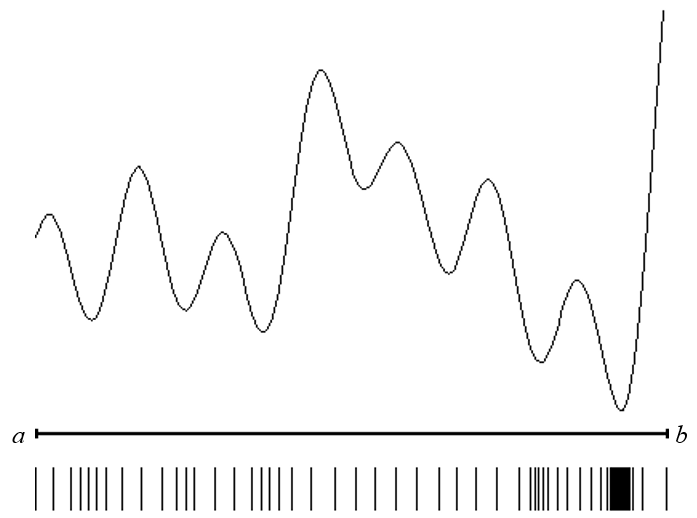
\includegraphics[width=0.8\textwidth]{figures/4_5.png}
  \caption{Minimization by means of Penalty Function Method}
\end{figure}

It is worth noting, that in the applied problems the estimates of the constraints as well as of the objective functions require considerable computation resources very often. The results presented in Table \ref{tab4:exp_results} confirm the effectiveness of the index scheme of the account of
constraints.

\begin{table}
  \caption{}
\begin{center}
  \label{tab4:exp_results}
  \begin{tabular}{| l | c | c | c| }
    \hline
    & $k_1$ & $k_2$ & $k_3$ \\ \hline
    Scanning a uniform grid & 160000 & 90280 & 56476 \\ \hline
    Penalty Function Method &  375 & 375 & 375 \\ \hline
    Index method & 63 & 49 & 35 \\ \hline
  \end{tabular}
\end{center}
\end{table}

Here $k_i$ is the number of computations of the $i$ problem function, i.e., of the function $g_i(x )$.
\begin{figure}[h]
  \label{fig:4_6}
  \centering
  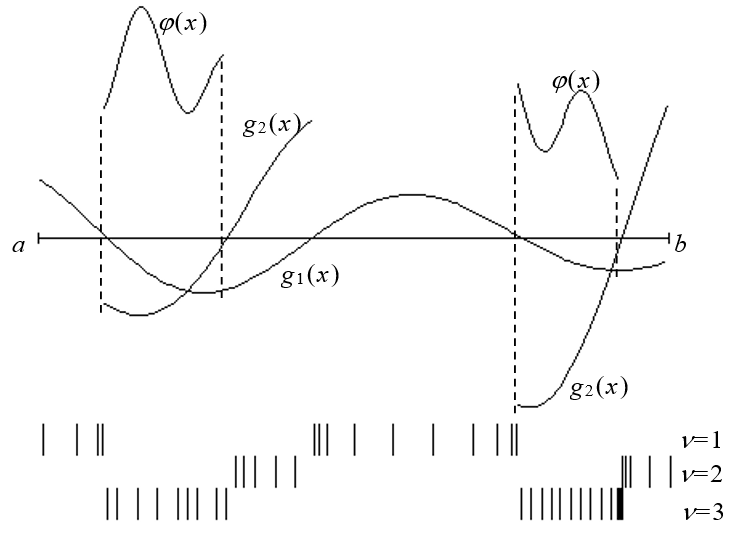
\includegraphics[width=0.8\textwidth]{figures/4_6.png}
  \caption{The minimization of an ''index'' function}
\end{figure}

\section{Index algorithm taking into account the existence of $\epsilon$-reserved solutions}
Let us return to the consideration of a one-dimensional problem of the kind \eqref{eq4:problem}
\begin{displaymath}
  \varphi(x^*)=\min\{\varphi(x):x\in [a,b], g_j(x)\le 0,1\le j\le m\}
\end{displaymath}
In the case when the objective function and the left-side parts of the constraints are partially computable, it is necessary to use the form \eqref{eq4:problem2}.
\example
{
Let us consider problem \eqref{eq4:problem} with $x\in[0,6,2,2]$, $m=3$ as an illustration:
\begin{gather}
\varphi(x)=\cos(18x-3)\sin(10x-7)+1, \\
g_1(x)=\exp(-x/2)\sin(6x-1.5) \\
g_2(x)=\sin(4x-2.2)+\cos(6x-2.9) \\
g_3(x)=|x|\sin(2\pi x - 0.5).
\end{gather}
}
\begin{figure}[h]
  \label{fig:4_7}
  \centering
  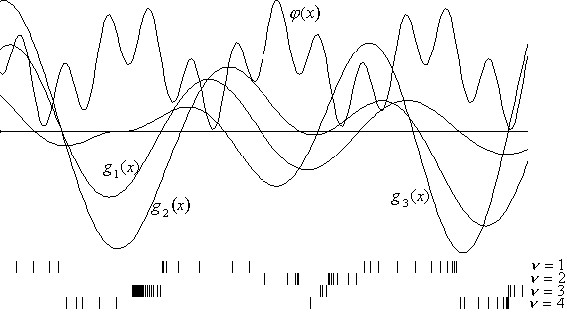
\includegraphics[width=0.8\textwidth]{figures/4_7.jpg}
  \caption{The solution of a problem by Index Method}
\end{figure}
The functions $g_j , 1\le j\le 4$, are pictured in Fig. \ref{fig:4_7}. Assuming a partial calculability, the arcs of
the functions corresponding to the domains $Q_j ,1\le j\le 4$, from \eqref{eq4:q} are presented in Fig. \ref{fig:4_8}.

\begin{figure}[h]
  \label{fig:4_8}
  \centering
  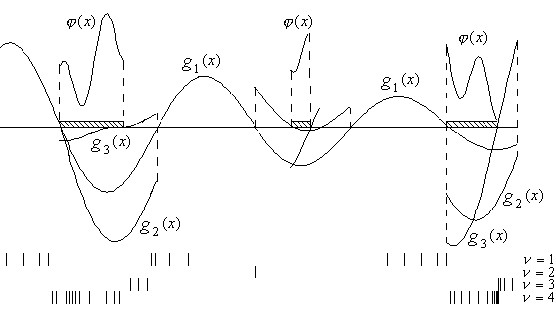
\includegraphics[width=0.8\textwidth]{figures/4_8.jpg}
  \caption{The problem solving by Index Method with the $\epsilon$-reservs}
\end{figure}

Index algorithm described in Sec. 3.3 was used to solve this example with $x_1=(a+b)/2$, $r=2$, and $\varepsilon=10^{-5}$. The coordinates of 102 trial points executed by the algorithm in the process of problem solving are marked by four rows of the vertical strokes in Fig. \ref{fig:4_7}. The strokes of the upper row correspond to the points with the index $\nu=1$, the ones of the second and the third rows --- to the points, the indices of which are equal to 2 and 3, respectively; and the points
marked by the strokes of the bottom row are feasible.

The coordinates of the trials executed in the close points are marked by a dark rectangle. The values of the functions $g_1 , g_2 , g_3$ , and $\varphi=g_4$ have been computed $k_1=102$, $k_2=80, k_3=64,$ and $k_4=26$ times, respectively. As one can see in Fig. \ref{fig:4_7}, the trial points concentration takes place not only in the vicinity of the point of the global optimum $x^*=2,07957$, but also in the vicinities of the inadmissible boundary points of the domains $Q_j$ from \eqref{eq4:q}. This effect can be reduced by the substitution of estimates \eqref{eq4:mu_const} by the estimates
\begin{equation}
  \label{eq4:mu_const}
  z_\nu^\ast = \left\{
  \begin{array}{lr}
    -\epsilon_\nu, & \nu < M,\\
    \min\{ g_\nu(y(x_i): i\in I_\nu \}, & \nu = M.
  \end{array}
  \right.
\end{equation}
where $\epsilon_R=(\epsilon_1 ,\dots, \epsilon_m)$ is a predefined vector with positive components. Thus, $z^*=0$ if there exist the points $x_i,1\le i\le k$ from series \eqref{eq4:search_data} with the index greater than $\nu$. As a consequence of this substitution the values of the characteristics $R(i)$ from \eqref{eq4:characteristic} will become lower (because of the subtraction of $\epsilon_\nu$) if
\begin{equation}
  \nu=\max\{\nu(x_{i-1},\nu(x_i)\}<\max\{\nu(x_j):1\le j\le k\}\le V
\end{equation}
that makes executing the trials in the corresponding intervals  ($x_{i-1}$ , $x_i$ ) less probable. In all other aspects, the algorithm remains the same.

This \emph{prima facie} mechanical trick has a well-established theoretical basis considered below.

\begin{definition}
  The point $x_\epsilon$ is called an $\epsilon$-reserved solution of problem \eqref{eq4:problem} if the condition
  \begin{equation}
    \varphi(x_\epsilon)=\min\{\varphi(x):x\in [a,b], g_j(x)\le -\epsilon_j,1\le j\le m\}
  \end{equation}
  meets where $\epsilon_1, \dots,\epsilon_m$ are the positive values of reserve for each constraint. Let us introduce into consideration also the set
  \begin{equation}
  X_\epsilon = \{x\in[a,b]:g_j(x)\le 0, 1\le j\le m, \varphi(x)\le\varphi(x_\epsilon)\}
  \end{equation}
  of all feasible solutions of the problem, which are no worse with respect to the objective function value than the $\epsilon$-reserved solution.
\end{definition}

The existence of the $\epsilon$-reserved solution of problem \eqref{eq4:problem} can be interpreted as some analogue of the conditions of regularity in the classical nonlinear programming problems. The applied role of this condition should be noted also. Even if the exact solution $x^*$ is known, its practical implementation is possible as some approximation to $x^*$ only. Therefore, the existence of the feasible points from $Q$ close to $x^*$ (with respect to the coordinates and to the objective
function values) is important. The existence of the $\epsilon$-reserved solution guarantees the availability of such points. Moreover, the domain $X_\epsilon$ may play a role of the set of suitable approximations.

The index algorithm with the $\epsilon$-reserves has been applied to the considered example with $\epsilon_i=0.2, 1\le i\le 3$. The search trial coordinates are marked by the vertical strokes in Fig. \ref{fig:4_8}. The solution has required 52 trials only and provided the same precision of the problem solution as in
the case when the vector $\epsilon_R$ equals to zero. Moreover, the values of the functions $g_1$ , $g_2$ , $g 3$ , and $\varphi=g_4$ have been calculated $k_1 =52$, $k_2 =39$, $k_3 =38$, and $k_4 =25$ times, respectively.

The conditions of convergence for the algorithm are presented in the following theorem (given without proof, see \cite{}).

\begin{theorem}
  Assume
\end{theorem}

\section{Index method with adaptive order of checking for constraints}
According to the rules of the index method considered in the preceding subsections, every trial includes the successive check of the fulfillment of the problem constraints in the corresponding point of the search domain. The finding of the first violated constraint terminates the trial and initiates the transition to the next iteration. If a numeration of the constraints in the increasing order by the computational costs of their checking is introduced (i.e., if the simpler constraints are checked first) one can reduce essentially the overall computational costs in the course of optimization. The above is important for the problems, in which the estimating of the function value requires a considerable computational resources connected with a necessity of the numerical modelling of the behavior of the systems described by these functions (as it takes place, for example, in numerous problems of the optimal design).

Obviously, the computational expenditures of the trial execution depend on the order of the problem functions’ computation essentially. If the calculation time of any problem is independent on the iteration execution point, the less the number of the problem functions (constraints and objective function) calculated at a point x, the less the trial execution costs in this point.

For many applied problems, it is naturally to assume that a constraint violated at a point in the search domain, will be violated in some neighborhood of this point as well. In this case, it might be useful to begin the next trials in the points of this neighborhood with checking the fulfillment of this particular constraint. In the scope of the above, it seems reasonable to design a global optimization algorithm allowing the modification of the constraint  check order taking into account the information obtained during the search. The check order design will be oriented onto the constraint violated at an iteration point to be found as early as possible.

\section{Parallel computations for the multiextremal optimization problems with nonlinear constraints}

\section*{A brief conclusion}
Constrained global optimization problems are under consideration. The method of penalty functions is one of the most popular numerical methods for solving the problems of this kind. Nevertheless, the method of penalty functions has a number of disadvantages. A new method for reduction of a constrained problem to an unconstrained one, so called \emph{index method}, has been considered in this chapter. This method, unlike the classical penalty function one, allows avoiding the problem of the parameter selection (like the penalty coefficients for the constraints). It is also allows solving the problems with partially defined objective function and constraints. This is quite natural for many applied problems, especially, in the optimal design of technical systems, because if some conditions of operation are not met, then some other characteristics of the system performance may not be defined.

The issues of convergence acceleration of the index method have been considered also. Two approaches for the convergence acceleration have been proposed. The first of them is based on concept of $\varepsilon$-reserved solution to the constrained problem. The role of $\varepsilon$-reserved solution in constrained global optimization problems is somewhat similar to the regularity requirements in classical nonlinear programming problems. The second approach is based on adaptive order of checking for constraints. In the index method, every iteration performed at the corresponding point of the search domain includes checking for constraints of the problem at this point. When a violation is discovered for the first time, the current iteration is stopped, and the next iteration is initiated. However, in Lipschitz optimization problems a constraint violated at a point of the search domain is also violated in a certain neighborhood of this point. In this case, to reduce the number of checks, it is expedient to begin iterations in the neighborhood of this point with checking for the violated constraint. Thus, the iteration can be completed at a lower cost.

For all proposed algorithms, the results of numerical experiments are presented. The results confirm the theoretical statements about convergence acceleration.

\end{document}
